% Options for packages loaded elsewhere
\PassOptionsToPackage{unicode}{hyperref}
\PassOptionsToPackage{hyphens}{url}
\documentclass[
]{ltjsarticle}
\usepackage{xcolor}
\usepackage[margin=20mm]{geometry}
\usepackage{amsmath,amssymb}
\setcounter{secnumdepth}{-\maxdimen} % remove section numbering
\usepackage{iftex}
\ifPDFTeX
  \usepackage[T1]{fontenc}
  \usepackage[utf8]{inputenc}
  \usepackage{textcomp} % provide euro and other symbols
\else % if luatex or xetex
  \usepackage{unicode-math} % this also loads fontspec
  \defaultfontfeatures{Scale=MatchLowercase}
  \defaultfontfeatures[\rmfamily]{Ligatures=TeX,Scale=1}
\fi
\usepackage{lmodern}
\ifPDFTeX\else
  % xetex/luatex font selection
\fi
% Use upquote if available, for straight quotes in verbatim environments
\IfFileExists{upquote.sty}{\usepackage{upquote}}{}
\IfFileExists{microtype.sty}{% use microtype if available
  \usepackage[]{microtype}
  \UseMicrotypeSet[protrusion]{basicmath} % disable protrusion for tt fonts
}{}
\makeatletter
\@ifundefined{KOMAClassName}{% if non-KOMA class
  \IfFileExists{parskip.sty}{%
    \usepackage{parskip}
  }{% else
    \setlength{\parindent}{0pt}
    \setlength{\parskip}{6pt plus 2pt minus 1pt}}
}{% if KOMA class
  \KOMAoptions{parskip=half}}
\makeatother
\usepackage{longtable,booktabs,array}
\newcounter{none} % for unnumbered tables
\usepackage{calc} % for calculating minipage widths
% Correct order of tables after \paragraph or \subparagraph
\usepackage{etoolbox}
\makeatletter
\patchcmd\longtable{\par}{\if@noskipsec\mbox{}\fi\par}{}{}
\makeatother
% Allow footnotes in longtable head/foot
\IfFileExists{footnotehyper.sty}{\usepackage{footnotehyper}}{\usepackage{footnote}}
\makesavenoteenv{longtable}
\usepackage{graphicx}
\makeatletter
\newsavebox\pandoc@box
\newcommand*\pandocbounded[1]{% scales image to fit in text height/width
  \sbox\pandoc@box{#1}%
  \Gscale@div\@tempa{\textheight}{\dimexpr\ht\pandoc@box+\dp\pandoc@box\relax}%
  \Gscale@div\@tempb{\linewidth}{\wd\pandoc@box}%
  \ifdim\@tempb\p@<\@tempa\p@\let\@tempa\@tempb\fi% select the smaller of both
  \ifdim\@tempa\p@<\p@\scalebox{\@tempa}{\usebox\pandoc@box}%
  \else\usebox{\pandoc@box}%
  \fi%
}
% Set default figure placement to htbp
\def\fps@figure{htbp}
\makeatother
\setlength{\emergencystretch}{3em} % prevent overfull lines
\providecommand{\tightlist}{%
  \setlength{\itemsep}{0pt}\setlength{\parskip}{0pt}}
\usepackage{bookmark}
\IfFileExists{xurl.sty}{\usepackage{xurl}}{} % add URL line breaks if available
\urlstyle{same}
\hypersetup{
  hidelinks,
  pdfcreator={LaTeX via pandoc}}

\author{}
\date{}

\begin{document}

\section{Paper 0.5: A Study of the Displacement-Record Mechanism ---
Recording of Displacement by Interference of ν Oscillation and the
Complex Plane, and the Composition of Two ±1/2
(±1)}\label{paper-0.5-a-study-of-the-displacement-record-mechanism-recording-of-displacement-by-interference-of-ux3bd-oscillation-and-the-complex-plane-and-the-composition-of-two-12-1}

\textbf{Author}: Noriaki Kihara \textbf{Affiliation}: WF System Co.,
Ltd.~/ ORCID: 0009-0004-6753-4020 \textbf{DOI}: Version
10.5281/zenodo.20689794 (this version) / Concept 10.5281/zenodo.20689793
(cite this; always resolves to the latest version) \textbf{Zenodo}:
https://zenodo.org/records/20689794 \textbf{Version}: v0.1 (definition
paper, first edition; settled after four review rounds judged ``ready to
submit''). Round 1: composition recast as interval arithmetic
(distribution assumptions dropped), arrow-of-time wording weakened,
notation t→φ, indistinguishability reframed as an information
projection. Round 2: φ fixed to the winding-number (progressive) reading
{[}reflection degeneracy made explicit, consistent with the sign
sector{]}, composition written as ``≤±1 is axiom-free / =±1 holds under
endpoint reachability'', the §2-phasor→§3-square-wave bridge and
edge-update rule made explicit, §3 split into derivation and Check 1
{[}boundary examples added{]}, a non-measurement disclaimer for
interference, and the Hartle analogy limited to slogan-sharing. Round 3:
the equal-frequency premise made explicit {[}the condition under which
the reflection degeneracy genuinely survives = the load-bearing point of
the Paper 13 link{]}, the equality condition corrected from
``independence'' to ``endpoint reachability'' {[}only anti-correlation
breaks it{]}, the scope of ``zero added axioms'' limited to the ±1
interval result {[}discrete sampling rests on the edge-update
modeling{]}, and the δ-unit commensuration of εx/εs made explicit. Two
optional sentences from Round 4 added. Two-party verification protocol.
\textbf{Type}: \textbf{Definition paper} (not an observation paper). It
introduces no new axiom; from the basic assumptions (2.5) and their
implicit definitions it defines the internal term ``displacement
record'' and verifies its properties by computation. \textbf{Series}:
The dual geometry of wavelength space and frequency space (Foundations
volume, Paper 0.5) \textbf{Verification script}:
\texttt{paper0\_5\_displacement\_record.py}

\begin{center}\rule{0.5\linewidth}{0.5pt}\end{center}

\subsection{0. Character of this paper --- what is defined and what is
not
claimed}\label{character-of-this-paper-what-is-defined-and-what-is-not-claimed}

This paper is a \textbf{definition paper} that, with \textbf{zero added
axioms}, makes precise the content of the words ``record,'' ``ledger,''
and ``register'' that the series has used.

State the important distinctions first.

\begin{itemize}
\tightlist
\item
  \textbf{We do not call it ``observation.''} Standard theory treats
  observation as an interaction with a measuring apparatus. Calling the
  present mechanism ``observation'' would invite the misreading ``one
  can observe without affecting the system,'' a denial of standard
  theory. This paper makes no such claim. What it defines is the
  internal term \textbf{displacement record}, and it does not enter the
  observation theory of standard physics.
\item
  \textbf{No new axiom is posited.} The axioms remain the basic
  assumptions 2.5 (νλ=1; zero-point δ=±1/2; asymmetric one bit). What
  this paper uses is only their \textbf{implicit definition} --- ν is
  the side measured as oscillation (the very meaning of ν=frequency in
  νλ=1).
\item
  \textbf{We do not use ``clock,'' ``monotone clock,'' ``entropy,'' or
  ``arrow of time.''} Time is a derived quantity in this series, and
  those words presuppose time, hence would be circular. This paper does
  not presuppose time; it goes only as far as showing that the
  displacement record fixes \textbf{distinguishability (the possibility
  condition for ordering)}. \textbf{The direction (arrow of time) is not
  derived here} --- orienting it would require the asymmetric one bit
  A3, which is outside the scope of this paper.
\end{itemize}

No physical identification is made.

\begin{center}\rule{0.5\linewidth}{0.5pt}\end{center}

\subsection{1. Basic assumptions and implicit
definitions}\label{basic-assumptions-and-implicit-definitions}

\textbf{Basic assumptions (2.5, common to the series)}

{\def\LTcaptype{none} % do not increment counter
\begin{longtable}[]{@{}ll@{}}
\toprule\noalign{}
\# & Assumption \\
\midrule\noalign{}
\endhead
\bottomrule\noalign{}
\endlastfoot
A1 & Reciprocal dual νλ=1 \\
A2 & Zero-point δ=±1/2 \\
A3 & Asymmetric one bit (which dual side carries conservation) \\
\end{longtable}
}

\textbf{Implicit definitions (contained in the meaning of νλ=1; not new
axioms)}

\begin{itemize}
\tightlist
\item
  \textbf{ν = the side measured as oscillation} (frequency). It is
  represented as a phase \(e^{i\varphi}\) on the complex plane (Argand
  plane). \(\varphi\) is the phase of the ν oscillation, not an external
  time.
\item
  The observable (state) is likewise represented as a phase
  \(z=e^{i\theta}\) on the same complex plane (amplitude normalized to
  1; the complex structure \(C\subset H\) of Paper 14). \(\theta\) is
  the phase of that observable. The appeal to Paper 14 plays only the
  light role of justifying ``amplitude 1, phase only''; the core of §2
  (\(|e^{i\theta}+e^{i\varphi}|^2\)) closes with elementary plane
  trigonometry alone.
\item
  \textbf{The observable \(x\) itself carries a ±δ ambiguity}: in this
  series the zero-point \(\delta=\pm 1/2\) (A2) is the minimal
  resolution, and any value carries a width of ±δ. Here we take
  \(\delta=1/2\) (A2 itself).
\end{itemize}

\begin{center}\rule{0.5\linewidth}{0.5pt}\end{center}

\subsection{2. Definition of the displacement
record}\label{definition-of-the-displacement-record}

Letting the observable's phase \(\theta\) interfere against the ν
oscillation \(e^{i\varphi}\) as reference, the interference intensity is

\[
I(\theta,\varphi)=\bigl|e^{i\theta}+e^{i\varphi}\bigr|^2=2\bigl[1+\cos(\theta-\varphi)\bigr]
\]

and \(I\) is determined by the relative phase \(\theta-\varphi\) alone.

\textbf{Fix the reading of φ uniquely.} In this series \(\varphi\) is
the \textbf{winding number (number of oscillations) = a progressive
phase}; at a single winding it takes a single intensity value (it is not
a spatial pattern running over a screen coordinate). Hence this paper
handles not ``fringe position,'' a spatial-pattern term, but \textbf{the
intensity value at a single winding}. Since \(\cos\) is even, a single
intensity value \(2[1+\cos(\theta-\varphi)]\) fixes only
\(|\theta-\varphi|\bmod 2\pi\); \(\theta-\varphi\) and
\(-(\theta-\varphi)\) cannot be told apart (\textbf{reflection
degeneracy}). Taking \(\varphi\) as a known, stable reference, what the
intensity value gives is ``\(\theta\) relative to \(\varphi\)'' up to
the ambiguity of reflection about the reference.

\textbf{The equal-frequency premise (the condition under which the
reflection degeneracy genuinely survives).} For the reflection
degeneracy to be true per-configuration, the reference \(\varphi\) and
the observable \(\theta\) must be \textbf{equal-frequency (with
\(\theta-\varphi\) constant in each configuration)}. The reason for
positing this, made explicit: if \(\theta\) is held fixed while
\(\varphi\) sweeps one turn, the maximum of the intensity
\(2[1+\cos(\theta-\varphi)]\) stands at \(\varphi=\theta\), so
\(\theta\) is read uniquely mod \(2\pi\) and the degeneracy disappears
(likewise two known reference values fix \(\theta\) via two equations).
Once equal-frequency is posited, each configuration yields a
\textbf{single stationary intensity value}, and sweeping across windings
in §3 yields no new information --- hence per-winding readout = full
information, and the reflection degeneracy survives true
per-configuration. When \(x\) changes stepwise, \(\theta\) jumps by
\(\Delta\theta\) to a new stationary value (level differences are
distinguishable; each level is reflection-degenerate). \textbf{This
reflection degeneracy is the same degeneracy as the series' sign sector
(Paper 13: position = sign sector)} and is consistent within this
paper's frame. Since a degeneracy that vanishes under sweeping could not
be identified with the sign sector, making equal-frequency explicit is
also the load-bearing point of this link.

Put differently, under equal-frequency \(\theta\) \textbf{co-rotates}
with \(\varphi\), and the observable \(x\) is \textbf{carried as the
constant offset \(\theta-\varphi\)} between them (\(x\) is not a
``static value'' but rides as a fixed difference against the progressing
\(\varphi\)). This single sentence makes explicit that the locked
interference reference of §2 (\(\theta-\varphi\) constant) and the
progressive sampling clock of §3 (edges defining the lattice) are
\textbf{two roles of the same \(\varphi\)}.

\begin{quote}
\textbf{On interference (disclaimer)}: the ``interference'' here is a
\textbf{formal construction} that fixes distinguishability, and does not
imply measurement by an apparatus (§5(i)). ``Intensity'' too is not an
instrument reading but the formal quantity
\(|e^{i\theta}+e^{i\varphi}|^2\).
\end{quote}

\begin{itemize}
\tightlist
\item
  \textbf{Configuration without change} (\(\theta=\) const): the
  intensity value does not change. No displacement is recorded.
\item
  \textbf{Configuration with change} (the two configurations \(\theta\)
  and \(\theta+\Delta\theta\)): the intensity values against the
  reference \(\varphi\) are \(2[1+\cos(\theta-\varphi)]\) and
  \(2[1+\cos(\theta+\Delta\theta-\varphi)]\), and for
  \(\Delta\theta\neq0\) they generically differ (except at the
  exceptional points of the reflection degeneracy). \textbf{That the two
  configurations give different intensity values is itself what makes
  them distinguishable} (we do not use the running word ``movement'' ---
  we state statically that the two configurations are distinguishable).
\end{itemize}

\begin{quote}
\textbf{Definition (displacement record)}: a \textbf{displacement
record} is the persistence in the structure of the observable's phase
difference \(\Delta\theta\) as a difference of interference intensity
values referenced to the ν oscillation \(\varphi\). If
\(\Delta\theta=0\) the intensity values coincide and no displacement
record arises. \textbf{Oscillation (ν) is the reference that makes a
displacement record possible; the change (\(\Delta\theta\)) is the
content of the displacement record.}
\end{quote}

\textbf{The displacement record gives the possibility condition for
ordering (distinguishability)}: for \(\Delta\theta\neq0\) the
configuration \(\theta\) and the configuration \(\theta+\Delta\theta\)
become distinguishable. But the set \(\{\theta,\theta+\Delta\theta\}\)
itself has no intrinsic \textbf{direction}. Which one is
``before/cause'' --- \textbf{the direction (arrow of time) is not
derived here} (just as Page--Wootters yields apparent correlations but
no arrow). Orienting it would require the asymmetric one bit A3, taken
to be outside scope. What this paper shows reaches only as far as a
change being \textbf{recorded in a distinguishable form} (the
possibility condition for ordering); time and clock are not presupposed.

\begin{center}\rule{0.5\linewidth}{0.5pt}\end{center}

\subsection{3. Derivation: two ±1/2 and the composition ±1 (interval
arithmetic)}\label{derivation-two-12-and-the-composition-1-interval-arithmetic}

\textbf{State first that §2 and §3 use different references.} The
reference of §2 is the fundamental phasor \(e^{i\varphi}\) (single
frequency, complex, continuous image), giving \(I=2[1+\cos]\). The
reference of this section is the limit taking \textbf{all of its odd
harmonics = the logic wave (square wave)}

\[
\nu(\varphi)=\frac{4}{\pi}\sum_{k\ \text{odd}}\frac{\sin(2\pi k \varphi)}{k}
\]

which is real-valued (converging to ±1, not \(e^{i\varphi}\)) and gives
ON/OFF (isomorphic to the logic wave of Paper 9: no amplitude, phase
only). Here \(\varphi\) is the winding number (number of oscillations),
not time. Note that the \textbf{reflection degeneracy established in §2
is a result of the fundamental phasor, and this section inherits it} ---
it is not re-derived anew with the square-wave reference (switching the
reference from phasor to square wave preserves the degeneracy, by
equal-frequency).

\textbf{State in one sentence the update rule that produces the discrete
sampling.} The square wave itself is a continuous function of
\(\varphi\) and does not, by itself, discretize. The discrete sampling
(cell width = 1 winding) arises when one posits the rule that
\textbf{the record is updated only at the ON/OFF edges (zero crossings)
of the logic wave}. Then the record-update points form a winding lattice
and the displacement record becomes \textbf{a discrete sampling per
oscillation}. That is, §2 (the continuous image treating the fundamental
as a phasor) → §3 (the odd-harmonic logic-wave limit, whose edges define
the winding lattice) is the bridge.

\begin{quote}
\textbf{Scope of ``zero added axioms'' (limitation)}: the ``zero added
axioms'' of this paper is a claim about the \textbf{±1 interval result}
below (A2 → interval sum, §3.1). The \textbf{discrete sampling
structure}, on the other hand, rests on the \textbf{posited update rule}
``update only at ON/OFF edges'' above, which is an additional modeling
choice not contained in A1--A3 nor in the implicit definitions (hence
the paper hedges with ``when one posits such a rule''). We make explicit
here the boundary between the theorem (zero axioms) and the
modeling-dependent structure.
\end{quote}

There are \textbf{two ±1/2 ambiguities} here.

\begin{enumerate}
\def\labelenumi{\arabic{enumi}.}
\tightlist
\item
  \textbf{Source-value ambiguity \(\varepsilon_x\)}: the observable
  \(x\) itself has a width of ±δ(=±1/2) (§1, the A2 zero-point). This is
  a quantity on the \textbf{value axis} (ambiguity of \emph{what}).
\item
  \textbf{Sampling ambiguity \(\varepsilon_s\)}: when \(x\) changes
  stepwise at a position off the winding grid, the discrete sampling
  rounds the change to ``the next winding'' = interval width 1 = ±1/2
  (Check 1). This is a quantity on the \textbf{winding axis} (ambiguity
  of \emph{when}).
\end{enumerate}

\textbf{On commensuration (why quantities on different axes can be
added).} \(\varepsilon_x\) (value axis) and \(\varepsilon_s\) (winding
axis) are conceptually quantities on different axes. They can be summed
into a single ±1 because A2 imposes \(\delta\) as a \textbf{universal
minimal resolution on all axes} (``any value carries ±δ''), so both axes
are commensurated in units of \(\delta\). Hence the interval sum
\([-\tfrac12,\tfrac12]+[-\tfrac12,\tfrac12]\) becomes well-defined (this
is the same commensuration implicitly used by ``ν itself is also ±1/2''
in §3.3).

\textbf{Check 1 (the ±1/2 of sampling,
\texttt{paper0\_5\_displacement\_record.py})}

{\def\LTcaptype{none} % do not increment counter
\begin{longtable}[]{@{}
  >{\raggedleft\arraybackslash}p{(\linewidth - 10\tabcolsep) * \real{0.1667}}
  >{\centering\arraybackslash}p{(\linewidth - 10\tabcolsep) * \real{0.1667}}
  >{\raggedleft\arraybackslash}p{(\linewidth - 10\tabcolsep) * \real{0.1667}}
  >{\centering\arraybackslash}p{(\linewidth - 10\tabcolsep) * \real{0.1667}}
  >{\raggedleft\arraybackslash}p{(\linewidth - 10\tabcolsep) * \real{0.1667}}
  >{\centering\arraybackslash}p{(\linewidth - 10\tabcolsep) * \real{0.1667}}@{}}
\toprule\noalign{}
\begin{minipage}[b]{\linewidth}\raggedleft
True change position
\end{minipage} & \begin{minipage}[b]{\linewidth}\centering
Record interval (n−1,n{]}
\end{minipage} & \begin{minipage}[b]{\linewidth}\raggedleft
Record-position estimate n−1/2
\end{minipage} & \begin{minipage}[b]{\linewidth}\centering
Ambiguity
\end{minipage} & \begin{minipage}[b]{\linewidth}\raggedleft
Error (est − true)
\end{minipage} & \begin{minipage}[b]{\linewidth}\centering
\textbar error\textbar≤1/2
\end{minipage} \\
\midrule\noalign{}
\endhead
\bottomrule\noalign{}
\endlastfoot
2.300 & (2,3{]} & 2.50 & ±0.5 & +0.200 & ✓ \\
5.700 & (5,6{]} & 5.50 & ±0.5 & −0.200 & ✓ \\
8.400 & (8,9{]} & 8.50 & ±0.5 & +0.100 & ✓ \\
2.999 (boundary) & (2,3{]} & 2.50 & ±0.5 & −0.499 & ✓ \\
3.001 (boundary) & (3,4{]} & 3.50 & ±0.5 & +0.499 & ✓ \\
\end{longtable}
}

The first three examples are near the cell center
(\(|\)error\(|\le0.2\)) and do not touch the upper bound. \textbf{±1/2
is the very definition of cell width 1}, not an upper bound the table
tested. The last two rows (boundary 2.999/3.001) confirm that the error
approaches the definitional upper bound ±1/2
(\(|{-}0.499|,|{+}0.499|<1/2\)).

\subsubsection{3.1 The composition is ≤±1 (axiom-free), =±1 (under
endpoint
reachability)}\label{the-composition-is-1-axiom-free-1-under-endpoint-reachability}

The record error is \(\varepsilon=\varepsilon_x+\varepsilon_s\). Here we
proceed in two stages, carrying this paper's own rigor standard all the
way.

\textbf{(a) The upper bound \(\le\pm1\) takes zero added axioms.} A2
says ``any value has a width of ±δ(=±1/2),'' so
\(|\varepsilon_x|\le\tfrac12\), \(|\varepsilon_s|\le\tfrac12\). By
subadditivity, with no assumption,

\[
|\varepsilon_x+\varepsilon_s|\le 1,\qquad\text{i.e.}\quad \mathrm{supp}(\varepsilon)\subseteq[-1,+1].
\]

This is a rigorous consequence of A2 alone, assuming neither a
distribution shape nor independence.

\textbf{(b) The equality \(=\pm1\) requires endpoint reachability (not
independence).} When both marginal supports are
\([-\tfrac12,\tfrac12]\), the support of the sum is
\(\mathrm{supp}(\varepsilon_x+\varepsilon_s)=\overline{\{a+b:(a,b)\in\mathrm{supp(joint)}\}}\).
The condition for this to reach all of \([-1,+1]\) is only that the
joint support reach the endpoints \((\tfrac12,\tfrac12)\) and
\((-\tfrac12,-\tfrac12)\) (i.e.~that both sources can simultaneously
take \(\pm\tfrac12\) in the same-sign direction, \textbf{endpoint
reachability}); the full rectangle is not required. Indeed:

\begin{itemize}
\tightlist
\item
  \textbf{Independent} (joint support = full rectangle) → \([-1,1]\) ✓
  (sufficient but not necessary)
\item
  \textbf{Perfectly positively correlated}
  (\(\varepsilon_x=\varepsilon_s\), joint support = diagonal) →
  \(a+b=2a\in[-1,1]\), all values reached ✓ (holds without independence)
\item
  \textbf{Perfectly anti-correlated} (\(\varepsilon_x=-\varepsilon_s\))
  → \(a+b\equiv0\), support \(=\{0\}\) × (the only type that breaks it)
\end{itemize}

That is, only \textbf{anti-correlation (endpoint avoidance)} shrinks the
support; positive correlation does not. So the equality condition is not
``independence'' but \textbf{endpoint reachability} (weaker than
independence, and favorable to this paper). Endpoint reachability is
\textbf{plausible} in this setting --- \(\varepsilon_x\) is the
resolution of the value, \(\varepsilon_s\) is the phase of the change
position against the grid, and there is no reason for the two sources to
be constrained to anti-correlation. Hence the conclusion (composition
±1) does not break. Since the word ``independence'' would reintroduce
probabilistic connotations into this paper's retreat from the
distribution layer to the support layer, we replace it, as a word too,
with endpoint reachability.

\begin{quote}
\textbf{Axiom-free \(\mathrm{supp}(\varepsilon)\subseteq[-1,1]\) (≤±1).
The equality \(\mathrm{supp}(\varepsilon)=[-1,1]\) (=±1) holds under
endpoint reachability.} This applies, one stage further to the equality
of the support, the same operation as the retreat performed in the
distribution layer (a triangular distribution requires independence +
uniformity → retreat to the support).
\end{quote}

\begin{quote}
\textbf{Note (the distribution shape is not a claim of this paper)}: if
\(\varepsilon_x,\varepsilon_s\) are assumed \textbf{independent and
uniform}, their convolution is the triangular distribution
\(f(\varepsilon)=1-|\varepsilon|\) on support \([-1,1]\) (standard
deviation \(1/\sqrt6\)). But ``independent'' and ``uniform'' are
\textbf{additional probabilistic assumptions} contained neither in
A1--A3 nor in the implicit definitions, and this paper does not use
them. This paper's claim stays at the \textbf{support} (≤±1 axiom-free,
=±1 under endpoint reachability) and does not enter the distribution
shape.
\end{quote}

\subsubsection{3.2 Indistinguishability (information,
projection)}\label{indistinguishability-information-projection}

What remains in the record is the composite
\(\varepsilon=\varepsilon_x+\varepsilon_s\) (one degree of freedom), and
\((\varepsilon_x,\varepsilon_s)\) (two degrees of freedom) is
\textbf{projected} onto this one degree. The projection kernel is
one-dimensional (the \(\varepsilon_x-\varepsilon_s\) direction), and
\((\varepsilon_x,\varepsilon_s)\) cannot be recovered from the record.
\textbf{Therefore whether the recorded ambiguity is ``sampling error''
or ``source-value ambiguity'' cannot be told apart} --- this follows,
independently of the distribution shape, from the structure alone of a
\textbf{2-DOF → 1-DOF projection (information loss)}.

\subsubsection{3.3 Treatment of ν, and the three-source case (interval;
an honest
statement)}\label{treatment-of-ux3bd-and-the-three-source-case-interval-an-honest-statement}

\begin{itemize}
\tightlist
\item
  \textbf{In this figure and section, ν itself is taken to be exact (no
  ±1/2 fluctuation), and the ambiguity of ν is omitted.} The ±1 in the
  figure is the composition of the \textbf{two} ±1/2 of source value and
  sampling (an interval sum under endpoint reachability).
\item
  For reference: if ν itself also had ±1/2, the interval sum would be
  \(3\times[-\tfrac12,+\tfrac12]=[-\tfrac32,+\tfrac32]\) = \textbf{±3/2}
  (not ±1). ``All of them ±1/2 → total ±1'' holds only for the
  \textbf{two-source case (source value + sampling)}; for three
  independent sources it is ±3/2.
\end{itemize}

\begin{figure}
\centering
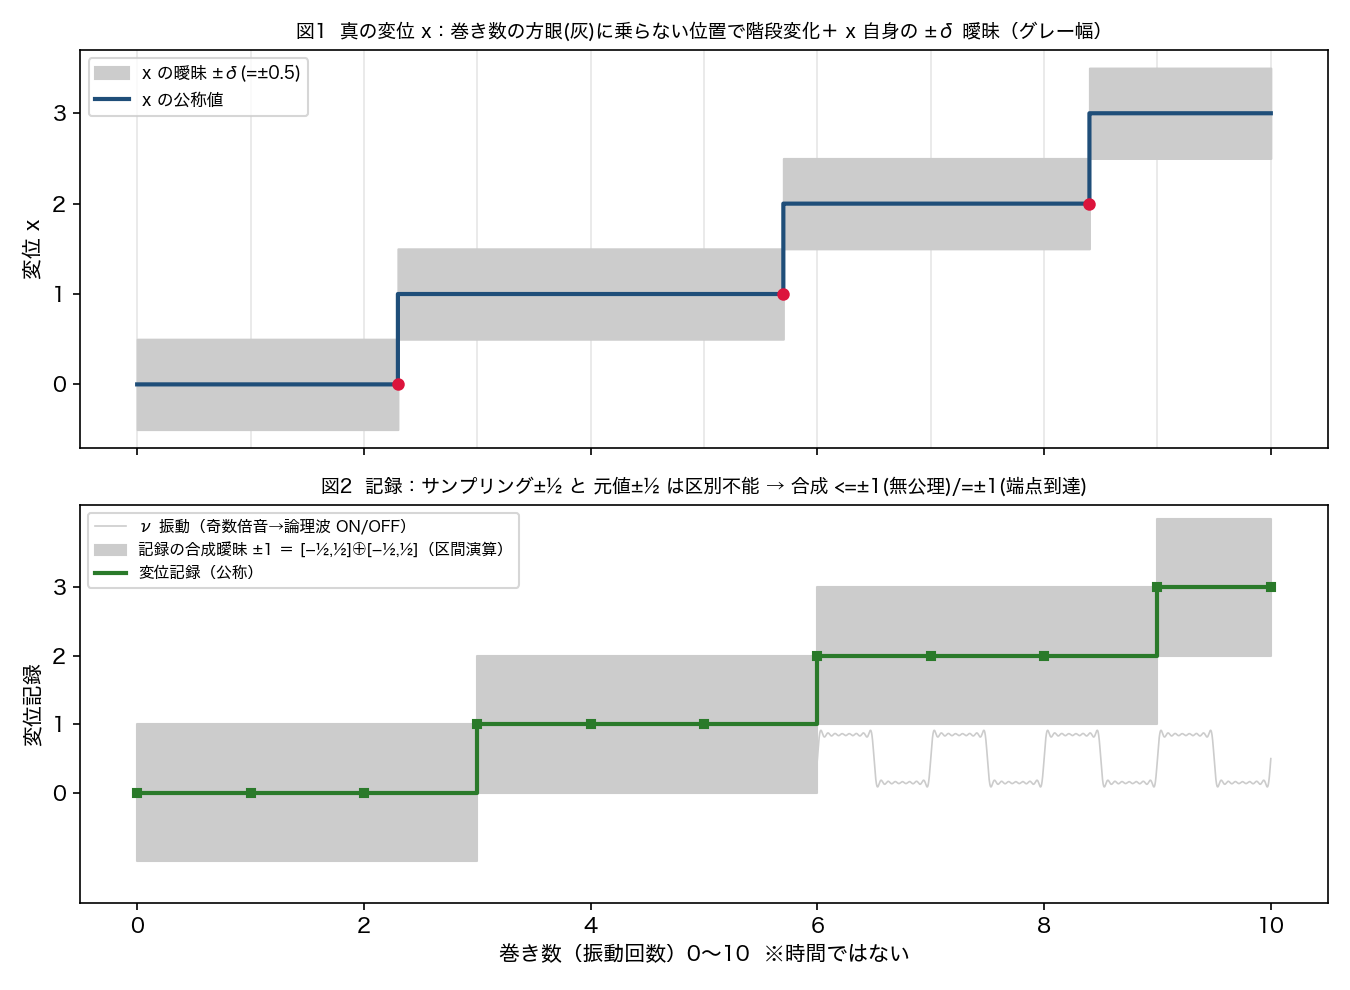
\includegraphics[width=0.92\linewidth,height=\textheight,keepaspectratio,alt={Displacement-record figure}]{paper0_5_fig_displacement_record.png}
\caption{Displacement-record figure}
\end{figure}

\textbf{Figure. The displacement-record mechanism (all exact interval
arithmetic, no schematics; the ambiguity of ν omitted).} \textbf{Top
(Fig. 1)}: the true displacement \(x\) changes stepwise at positions off
the winding grid (gray lines) (2.3, 5.7, 8.4), and \textbf{\(x\) itself
carries a ±δ(=±0.5) ambiguity (gray band)}. \textbf{Bottom (Fig. 2)}:
the displacement record (green) sampled by the ν logic wave (odd
harmonics → ON/OFF, gray). \textbf{Source-value ±1/2 and sampling ±1/2
are indistinguishable, and the composition is axiom-free ≤±1, =±1 under
endpoint reachability (gray band)}. The horizontal axis is the winding
number (number of oscillations), not time.

\subsection{4. Connection to existing papers (tidying the
nomenclature)}\label{connection-to-existing-papers-tidying-the-nomenclature}

By the present definition, the words of existing papers are tidied as
follows (content and results are unchanged; this is a tidying of
nomenclature).

\begin{itemize}
\tightlist
\item
  \textbf{Places that used ``ledger'' / ``register'' in the sense of the
  entity of the record (the side that holds change)} →
  \textbf{displacement record} (the defined term of this paper).
\item
  Places that meant the conserved quantity (\(\sum\nu^2\)) →
  \textbf{conserved quantity} (not a displacement record = the side that
  cannot be recorded).
\item
  Places that meant the invariant coordinates \((R,Q)\) →
  \textbf{invariant (coordinates)}.
\item
  Places that meant the count of degrees of freedom → \textbf{count of
  degrees of freedom / number of conservation laws}.
\end{itemize}

Thereby the hitherto-ambiguous ``ledger/register'' is sorted into either
the \textbf{defined displacement record} or \textbf{plain mathematical
terms (conserved quantity, invariant)}, removing a source of misreading.

\begin{center}\rule{0.5\linewidth}{0.5pt}\end{center}

\subsection{5. What is not claimed}\label{what-is-not-claimed}

\begin{enumerate}
\def\labelenumi{(\roman{enumi})}
\tightlist
\item
  Observation (interaction with a measuring apparatus) --- not discussed
  here. The displacement record is an internal term, not an observation
  theory.
\item
  New axioms --- none posited (the basic assumptions 2.5 stand; only the
  implicit definitions are used).
\item
  Clock, monotone quantity, entropy, arrow of time --- not used (to
  avoid the circularity of presupposing time).
\item
  The fluctuation of ν itself --- omitted here as exact (§3.3). The ±1
  in the figure is the composition of the two ±1/2 of source value and
  sampling.
\item
  Physical identification.
\end{enumerate}

Time, ordering, and causality are \textbf{derivatives} of the
displacement record (the detection of \(\Delta\theta\)).

\begin{center}\rule{0.5\linewidth}{0.5pt}\end{center}

\subsection{Relation to prior work (external, minimal,
verified)}\label{relation-to-prior-work-external-minimal-verified}

The series' policy is not to cite external literature, but because this
paper, by its nature, honestly makes explicit its relation to the
adjacent notions of ``record'' and ``time is not fundamental,'' it
carries a minimal set of external references (conceptual background, not
the basis of this paper's definition). \textbf{The displacement record
is the defined term of this paper, not an established term.} The
relations to adjacent notions are stated below, distinguishing
slogan-sharing from whether the content is implemented.

\begin{itemize}
\tightlist
\item
  That time is not a fundamental degree of freedom but emerges from
  correlation/reference: D. N. Page, W. K. Wootters, ``Evolution without
  evolution: Dynamics described by stationary observables,'' \emph{Phys.
  Rev.~D} \textbf{27}, 2885 (1983), DOI 10.1103/PhysRevD.27.2885. This
  paper's character --- ``the possibility condition for ordering arises
  from correlation with a reference, but the direction (arrow) does
  not'' --- is precisely isomorphic to Page--Wootters.
\item
  A formulation that starts from records: J. B. Hartle, ``Decoherent
  Histories Quantum Mechanics Starting with Records of What Happens,''
  arXiv:1608.04145 (2016). This paper \textbf{shares} Hartle's slogan
  ``start with records'' but \textbf{does not implement} decoherent
  histories --- it has no decoherence functional, no consistency
  condition, no environment, no quasiclassical domain. We limit this to
  sharing the slogan, not implementing the content.
\item
  The logic wave (the odd-harmonic square wave): Paper 9 of this series.
\end{itemize}

\begin{center}\rule{0.5\linewidth}{0.5pt}\end{center}

\textbf{Acknowledgment / procedure}: the definition and verification of
this paper follow a two-party verification protocol by Claude Code
(local machine verification) and claude.ai (independent computation and
review). The verification script
\texttt{paper0\_5\_displacement\_record.py} is bundled. No physical
identification is made.

\end{document}
